\RequirePackage{fixltx2e}
\documentclass[a4paper, titlepage, 12pt, twoside, open=right]{scrartcl}
\usepackage[utf8]{inputenc}  
\usepackage[T1]{fontenc}
\usepackage{mathtools}
\usepackage{longtable}
\usepackage{lmodern}           
\usepackage{polyglossia}
\usepackage{morewrites} %wtf
\usepackage{forest} % this is for the stemma diagram
\usepackage[onehalfspacing]{setspace}
\usepackage[toc,page]{appendix}
\usepackage{multirow,bigdelim}
\usepackage{parnotes}
\usepackage{xfrac}
\usepackage{graphicx}% stellt \scalebox bereit
\usepackage{array,booktabs}% für Tabellen
\usepackage{natbib}
\onehalfspacing
\setdefaultlanguage{english}
\setotherlanguage{hindi}
\setotherlanguage{tibetan}
\newfontfamily\tibetanfont{Tibetan Machine Uni}
\usepackage{xeCJK}
 \setCJKmainfont[BoldFont=SimHei]{SimSun}
%\setCJKmainfont{Noto Sans CJK TC Regular}
\usepackage{marginnote}
\font\tibfont="Tibetan Machine Uni" at 11 pt
\usepackage{geometry}           
\usepackage[multiple,perpage]{footmisc}
\usepackage{endnotes}
\def\enoteheading{\section{\notesname}%
\mbox{}\par\vskip-\baselineskip}
\geometry{left=2cm,right=3cm,top=2.5cm,bottom=2.5cm}
\usepackage{changepage}
\usepackage[hidelinks]{hyperref}
\usepackage{xcolor}

%avoid indent in quotes:
\makeatletter
\renewenvironment{quotation}
  {\list{}{\listparindent=1.5em
           \itemindent=0pt
           \parsep\z@ \@plus\p@}%
           \item\relax}
  {\endlist}
\makeatother



\begin{document}

% %\pagestyle{normal}
\clearpage
\thispagestyle{empty}
\titlehead{DRAFT}
\title{A statistical analysis of word-lengths in the Pali canon}
\subtitle{}
\author{Venerable Vimala Bhikkhunī}
\date{\today}
\maketitle

\tableofcontents
\newpage
\section{Summary}
The Pali language, as every other language, has evolved over time. One of the changes that the language has undergone through the centuries is that words have become increasingly complex and words have merged together to form longer words. We would therefore expect that a statistical analysis of average word-length could be an indication of relative "age" of the texts in question. 

In this research I analyse the average word-length of each text and each book in the Pali canon to find trends in the canon and test the above hypothesis; to show that average word-length can be used as an indicator to show the development of the texts over time.\\

Average word-length in itself remains only an indication of "lateness" of texts, among other indications like the existence and quality of parallels, but nevertheless can prove a valueble resource in determining the development of the texts in the Pali canon and ultimately what the Buddha taught.

The analysis of word-length is more reliable on larger texts, or whole collections and books, than it is on individual texts; if texts are heavily abbreviated or consist only of a few lines, the word-length can give a value that is not representative of the collection as a whole and can greatly vary.

\newpage
\section{Methodology}
\subsection{Sourcing texts}
For this research, I used the Pali canon from the Mahāsaṅgīti Tipiṭaka Buddhavasse 2500 from the Vipassana Research Institute (\url{https://tipitaka.org/}).

These texts, with the exception of the commentarial texts, are used by SuttaCentral.net and they have partly segmented these files and coded them in json. These json files do not have any of the coding that is necessary to display texts online but just the pure texts, which makes it ideal to work with. This format is the basis I used for my analysis.

Where these files did not exist, I have taken them from the SuttaCentral HTML and coded them into the same segmented json format. The same I have done for the commentarial texts directly from the VRI website in XML.

The github repository for these json files is here: (\url{https://github.com/BuddhaNexus/segmented-pali})

\subsubsection{Variant readings}
The Mahāsaṅgīti Tipiṭaka as used by the VRI as well as SuttaCentral also list various variant readings. These were removed for the purpose of this analysis. After analysing part of the variant readings I concluded that these would not make a significant shift in the calculations. In some cases variant words were a bit longer, in other cases shorter.

\subsubsection{Abbreviations}
Many texts contain abbreviations in the form of "… pe …" or similar. These abbreviations were removed prior to calculations because they would give a much lower average word-length for texts with many abbreviations. Of course this will go from the premise that the text being substituted has an overall average that is roughly the same as the still remaining text. I feel this is reasonable assumption and above all, it would be undo-able to replace the abbreviations with the text they are to replace.

\subsection{Other materials used}
In some instances I had to look into the parallels distribution of files within a collection. For this I used the parallels json file that is used by SuttaCentral. Although this material is not complete i.e. these are human sourced parallels and not all parallels will be known, they give an indication. Moreover, these parallels also list known parallels with other Buddhist canons in other languages.

One major drawback in using this parallels-list for statistical analysis is that it is not consistent in how it counts parallels. For instance text A can be parallel to text B and this can list as one parallel. But it is also possible that a more detailed listing is applied in that for instance text A, verse 1 is parallel to text B, verse 2, etc. This multiplies the number of parallels considerably. 

In analysing some collections, I also made use of a sankey map and other graphs as used by BuddhaNexus.net. Although this is very detailed and complete, it only lists matches within the same canon. Matches within the same canon have their value, but in matching between various languages we can determine if texts were already in existence before the split of the schools and therefore their relative age (see \citep{sujatobrahmali}). The matching between languages is in the pipeline but to date not yet available. 

Note also that BuddhaNexus graphs show the total lengths of matches so that a long match between texts counts for more than just one line, as opposed to the parallels listed in SuttaCentral, where every match just counts as 1. Therefore, it also takes the quality of the match into account.

\subsection{Method of analysis}
The segmented files were further imported into an ArangoDB database and queries made from there, using the Python programming language for retrieving meaningful data for barcharts.

All punctuation and other typography markers and numbers were removed so only the alphanumerical characters were used for calculating the average word-length.

\newpage
\section{Average Word-length (AWL) analysis}
\subsection{First results}
After calculating and plotting the average word-length (hereinafter called AWL) of all collections in the Pali canon, the following chart ensued:\\

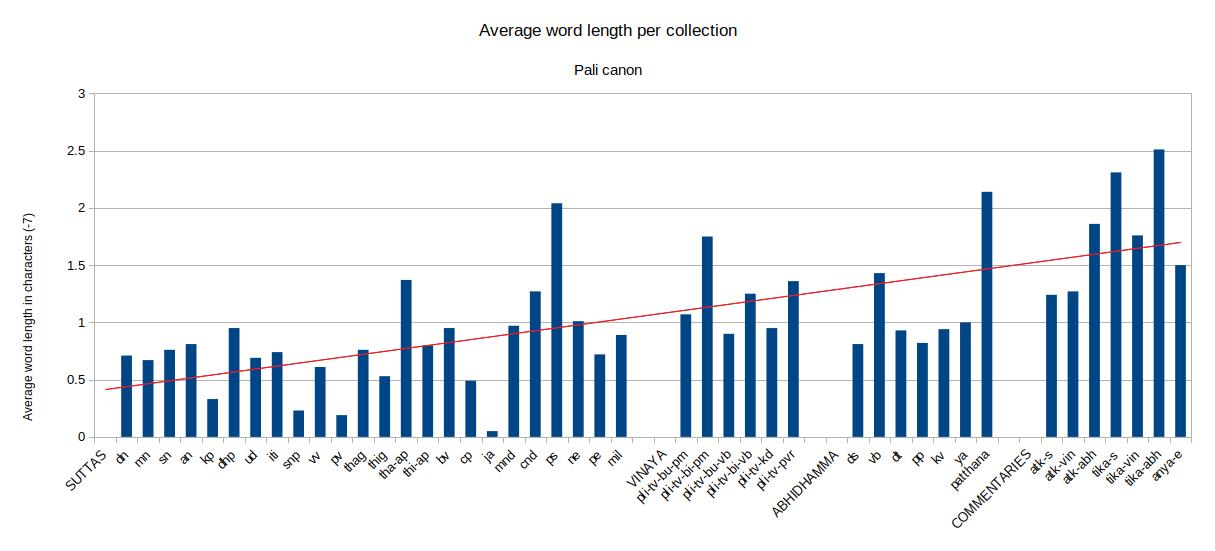
\includegraphics[width=\linewidth]{chart1.jpg}
\captionof{figure}{The AWL in characters above 7 per collection in the Pali canon. The red line shows the linear trendline (regression through equation y=a*x+b)}
\label{chart1}

\medskip
Some interesting things can be seen from this chart. First of all, it is clear that most collections that are generally accepted as "Early Buddhist Texts (EBTs)"--the first four Nikāyas and the first 9 collections in the Khuddaka Nikāya with the exception of the Vimānavatthu and Petavatthu (see \citep{sujatobrahmali})--have a lower AWL while the later commentarial texts have a much higher AWL.

The Vinaya and Abhidhamma texts as well as the later Sutta texts seem to be in between with roughly the same range of AWL, indicating that these texts might have developed over a period of time thereafter. There are also some collections that do not match this broad pattern and I will discuss these below.

Especially the relative high value of the Dhammapada (dhp) is surprising because the Dhammapada is generally seen as one of the earliest Buddhist texts. Then there are other discrepancies like the Jātaka (ja) and the Bhikkhunī Pātimokkha (pli-tv-bi-pm). So I will explore these in more detail below.

\subsection{The influence of headings}
Analysing the Dhammapada (dhp) (\url{https://suttacentral.net/dhp/pli/ms}), I noticed that especially the headings have a much larger word-length than the verses. 

If we keep in mind that all early texts were only transmitted orally and organized and written down at a much later date, it is likely that headings were inserted into the texts later, when these texts were scripturalized.

So calculating the same chart with the headers removed gives the following interesting picture:\\

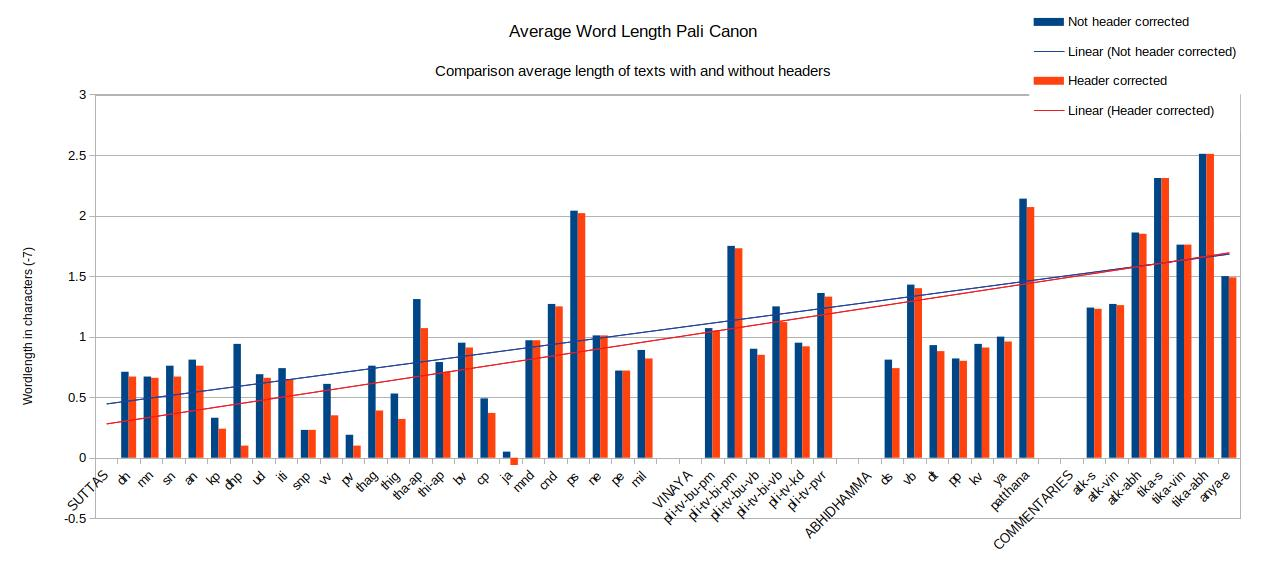
\includegraphics[width=\linewidth]{chart2.jpg}
\captionof{figure}{The AWL in characters above 7 per collection in the Pali canon comparing calculations with and without headers. The blue and red lines shows the linear trendlines resp. (regression through equation y=a*x+b)}
\label{chart2}

\medskip
Removing headers from the calculation and just analysing the prose or verse text suddenly gives a very different picture for expecially the Dhammapada, which has now jumped from a relatively high value to a much lower value which is much more in line with our accepted understanding of the Dhammapada as a very early text.

Another interesting thing we see in this chart is that removing the headers has a much more dramatic effect on the Early Buddhist texts and the commentarial texts are hardly affected. So I think it is safe to assume that headers are indeed inserted into the texts later.

\subsection{Verse vs. prose}
When we look at the early Buddhist collections, the EBTs, we notice another interesting phenomenon: collections with predominantly verses have a much lower AWL than collections with prose, also those that are regarded as "late".

There are various ways in which this can be explained. First of all, it might be that verse, by its very nature, needs shorter words. But this is not always the case.

Another possibility is that due to the history of oral tradition, it was much easier to remember and recite verses than prose and we do indeed see that verse summaries of prose teachings were one method to ensure oral transmission.

In the following chart we can see this difference a bit more clearly, using a different scale to the previous charts. Here the y-axis shows the AWL in characters above 7.76 so the EBT collections all get a negative value.\\

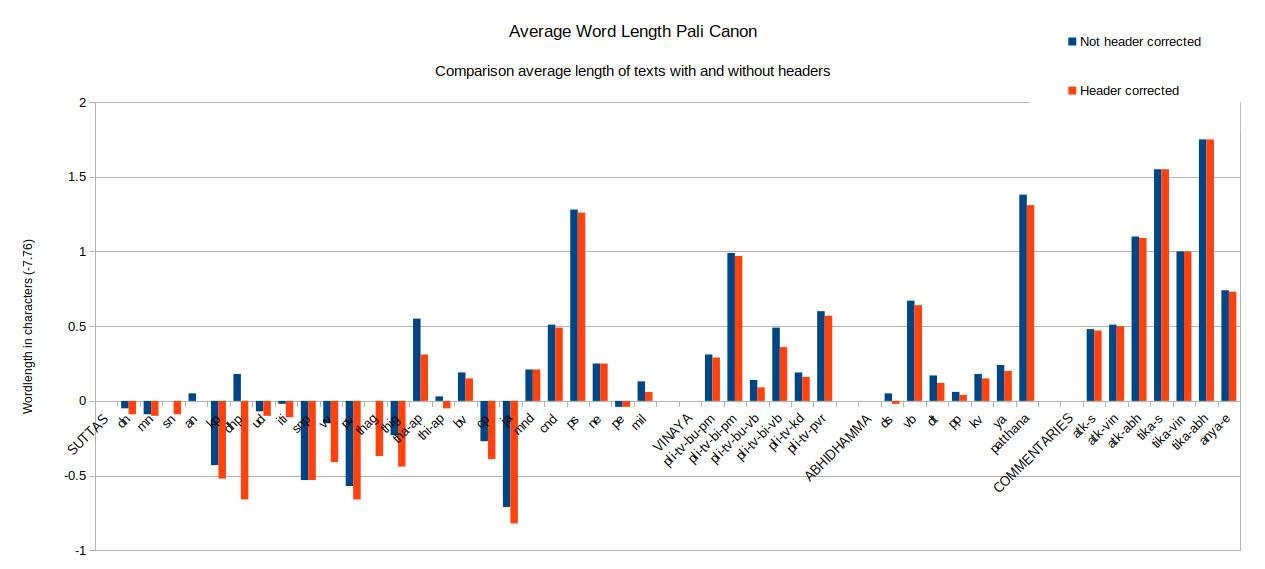
\includegraphics[width=\linewidth]{chart3.jpg}
\captionof{figure}{The AWL in characters above 7.76 per collection in the Pali canon comparing calculations with and without headers. The blue and red lines shows the linear trendlines resp. (regression through equation y=a*x+b)}
\label{chart3}

\medskip
The value of 7.76 is chosen because this is the highest value for the AWL of all the EBTs, corrected for headers. This is, maybe not surprisingly, the value of the Aṅguttara Nikāya. This value is consistent with our understanding that from all the EBTs the Aṅguttara Nikāya has been influenced most by later insertions.

\subsection{Collections with a very high or low value}
There are several collections that show a surprising high or low value of AWL in the chart and I will analyse each of these below.

\subsubsection{Jātaka (ja)}
One of the most striking anomalies is the Jātaka collection. In fact, it is the collection with by far the lowest AWL.

This is a collection of 547 sets of verses. The canonical Pali collection consists of verses arranged in numbered sets; the shorter sets illustrate a high point of a story, while the longer sets tell a complete story. These verses would have been passed down from the beginning with prose narrative to flesh out the story, which in the Pali is now found in the commentary. 

The Jātaka verses are generally seen as pre-Buddhist tales. They came into the Buddhist canon, not only because the Buddha himself sometimes used these tales in his teachings, but also because the old tales would get a story woven around them in which these were said to be the stories of the Buddha's previous lives. However, these prose stories are not in the canonical collection of the Jātaka, where only the verses are used. The prose stories were added only in the commentaries. 

So it is maybe not so surprising that these stem from an earlier use of the Pali language and therefore have a shorter overall word-length. However, this does not explain the very low AWL value of some of the other late verse-collections.

The below figure shows the distribution of the Jātakas.\\

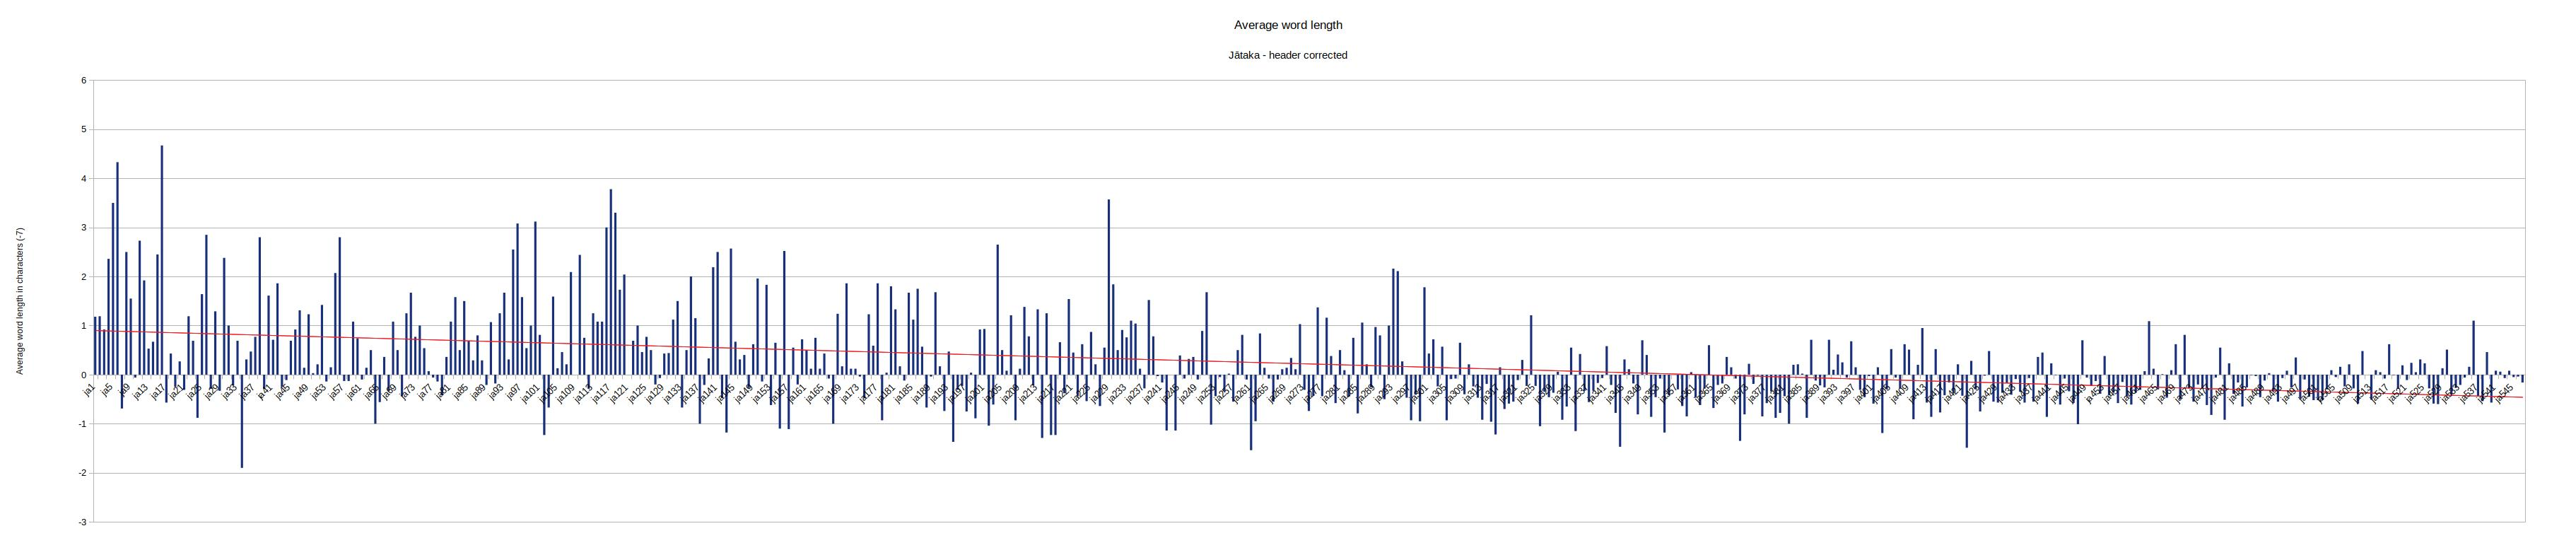
\includegraphics[width=\linewidth]{jataka.jpg}
\captionof{figure}{The AWL in characters above 7 per collection in the Pali canon comparing calculations with and without headers. The red line shows the linear trendline (regression through equation y=a*x+b)}
\label{jataka}

\medskip
This figure shows an interesting trend: the shorter Jātakas with a lower number seem to have a much higher word-length on average than the ones further in the collection. 

The next figure shows the number of parallels listed on SuttaCentral for the texts in this collection on a logarithmic scale. \\

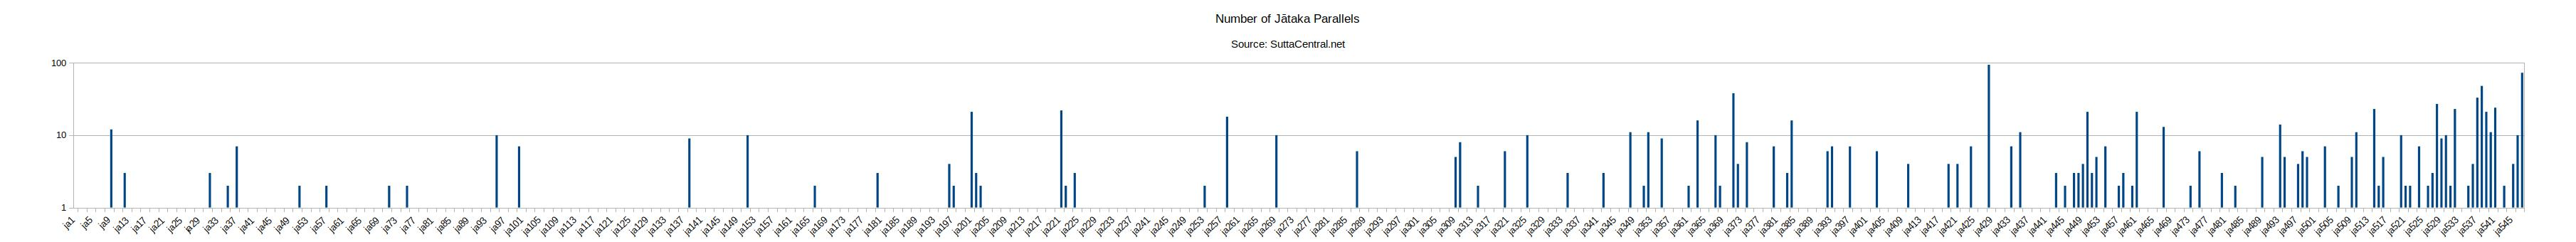
\includegraphics[width=\linewidth]{jatakapars.jpg}
\captionof{figure}{The number of parallels as listed on SuttaCentral on a logarithmic scale}
\label{jatakapars}

\medskip
Although there are not very many known parallels for many of these texts, it is clear from this that the most parallels appear in the higher end of the Jātaka collection, where the complete story is told.

From both of these charts it would seem that the Jātaka with a higher number are likely to be earlier than the first part of the collection. Of course we cannot make any assumptions about the lateness or earlyness of individual suttas based on this method, especially if many of these only contain just one verse, but it is an indication of a general trend.

\subsubsection{Vimānavatthu (vv) and Petavatthu (pv)}
The most striking about the Vimānavatthu and Petavatthu is that they seem to fit seemlessly into the graph as part of the EBTs according to their AWL. Yet they are generally accepted to be late devotional texts with no direct counterparts in other collections.

In how far the low AWL value has to be sought in the fact that these are verse collections I cannot tell. Another possibility is that in order to be consistent, the authors of these texts have gone through considerable length to use a language that was more consistent with the early texts; it might be an attempt to make the texts look genuine. More research will need to be done to find an answer to this question.

\subsubsection{Therāpadāna (tha-ap) and Therīapadāna (thi-ap)}
These are later texts that lack counterparts in the northern canons. In analysing this text I can find no reason for the relatively low value of the AWL for the Therīapadāna in comparison to the Therāpadāna. It seems however that the last part of the Therāpadana is slightly lower in AWL and more consistent with the low value of the Therīapadāna.

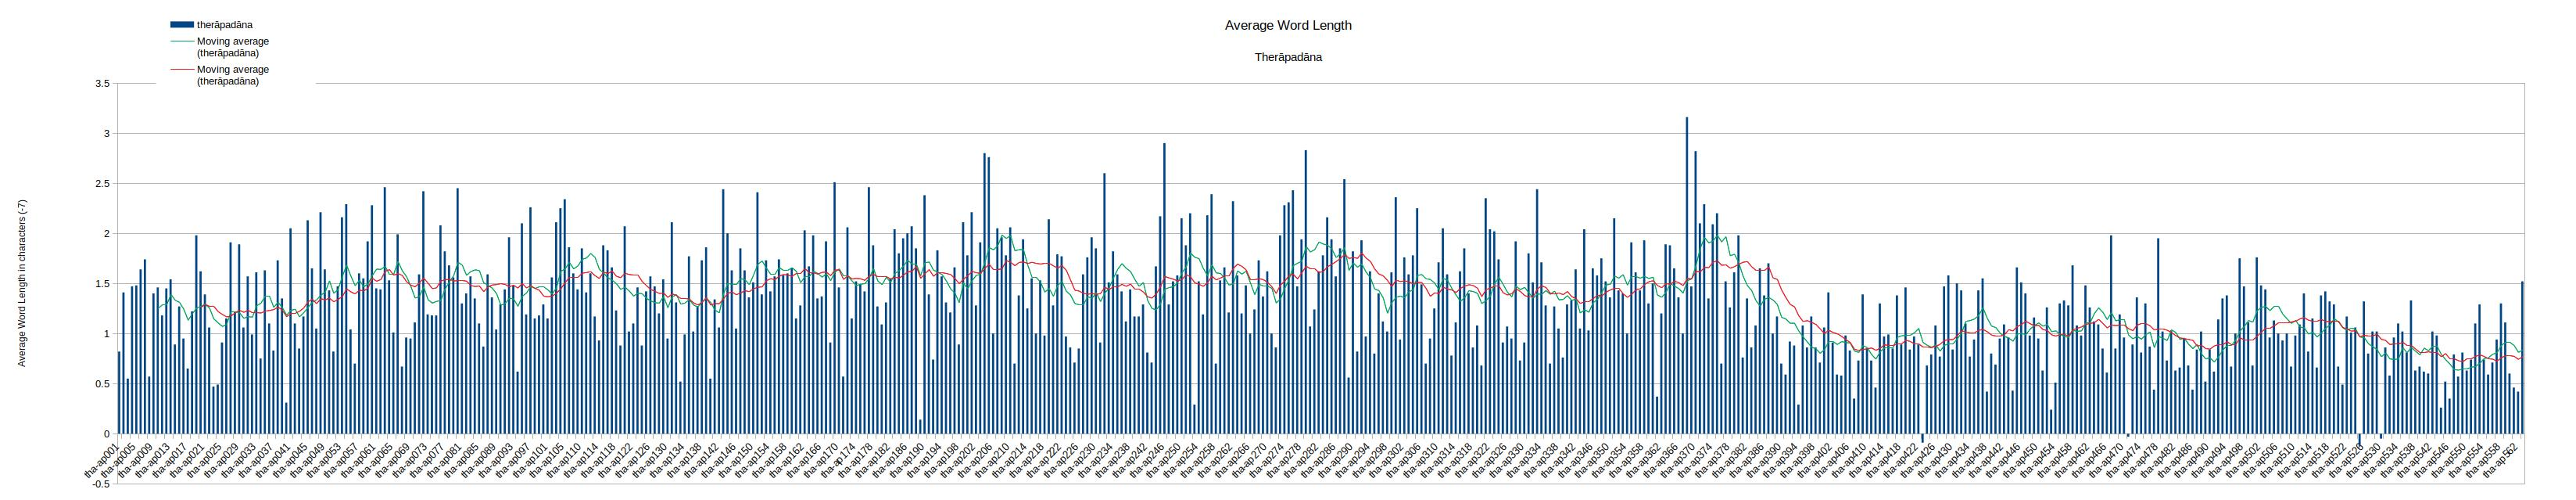
\includegraphics[width=\linewidth]{thaap.jpg}
\captionof{figure}{Therāpadāna AWL values with moving average lines (green = period 10, red = period 20)}
\label{thaap}

\medskip
Around the Pilindavaccha Vagga the AWL value makes a drop as is also clear from the moving average lines. From this point onwards, the AWL values of the Therāpadāna are much more consistent with the Therīapadāna as the following chart shows. This might indicate that these parts are slightly earlier and that the first parts of the Therāpadāna (with shorter texts) was added later.\\

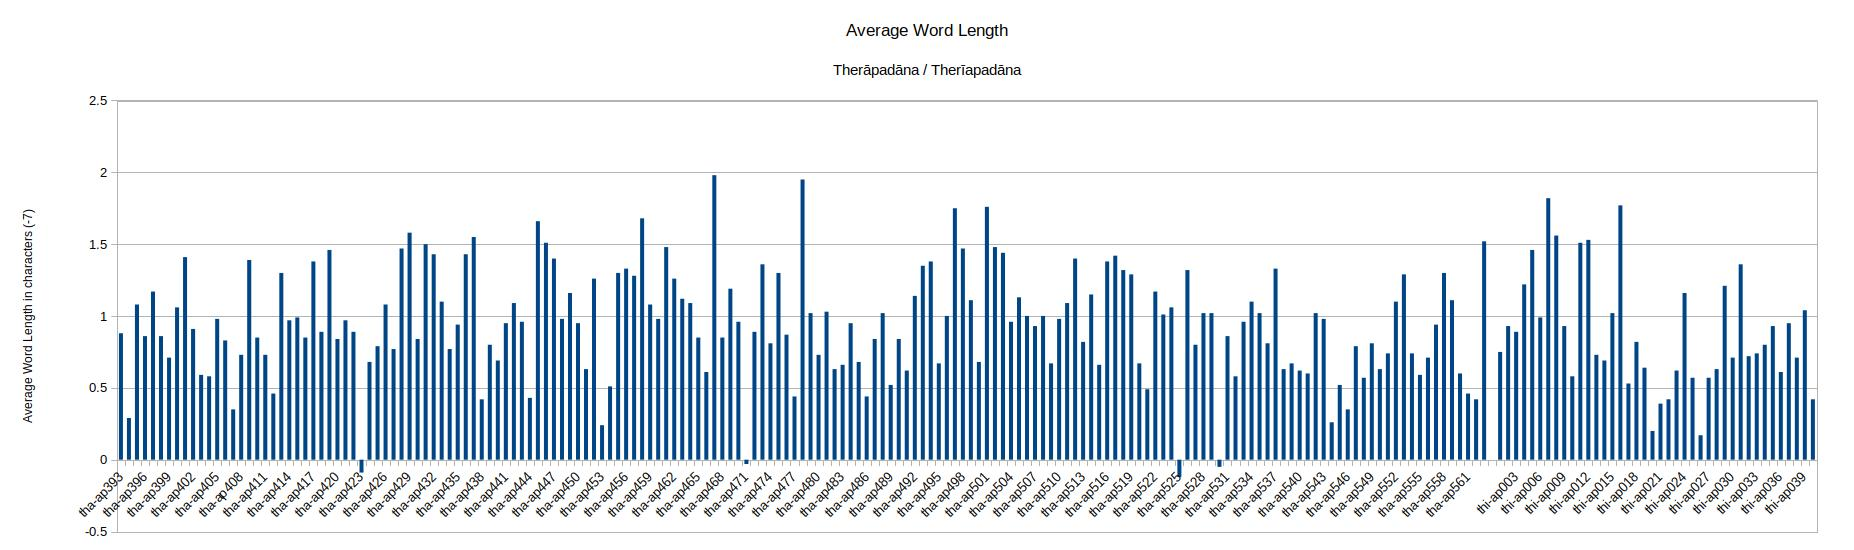
\includegraphics[width=\linewidth]{thaiap.jpg}
\captionof{figure}{Therāpadāna AWL from Pilindavaccha Vagga onwards in comparison to the Therīapadāna}
\label{thaiap}

\subsubsection{Cariyāpiṭaka (cp) and Buddhavaṃsa (bv)}
Another interesting collection as is seen in figure \ref{chart3} is the Cariyāpiṭaka. A small collection of only 35 verse-texts, it mainly comprises of retellings of the Jātaka stories. It represents an early systematization of the concept of the Bodhisattva and his path towards awakening. It is a late text, without direct counterparts in the northern collections. Like the Buddhavaṃsa, it is part of an extensive pan-sectarian devotional literature composed in the second and first centuries BCE, presaging the birth of the Mahāyāna.

Analysing this in a chart we get the following:\\

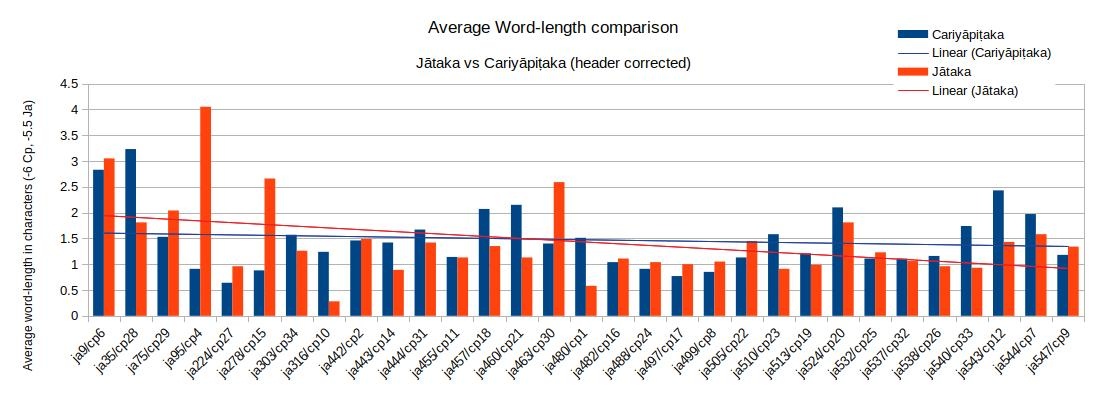
\includegraphics[width=\linewidth]{jacp.jpg}
\captionof{figure}{Comparison of Jātaka with Cariyāpiṭaka (Note that for the purpose of this comparison the value of length for Cariyāpiṭaka is .5 characters higher than for Jātaka)}
\label{jacp}

\medskip
There seems to be a rough, but not entirely convincing, similar trend between the two collections. More notably we see that most of the Cariyāpiṭaka are retellings of the Jātaka with higher numbers. 

Although at present I do not have a convincing explanation as to why the Cariyāpiṭaka, unlike the Buddhavaṃsa, would have such a very low AWL, given it's age but I suspect it's correlation to the Jātaka might have something to do with it.

Both collections are vastly different from the other collections. The sankey charts below show there are no matches found between them and other collections, indicating a completely different use of language. The same pattern we also see for the Therāpadāna, Theriapadāna and to a lesser extend for the Vimānavatthu and Petavatthu.\\

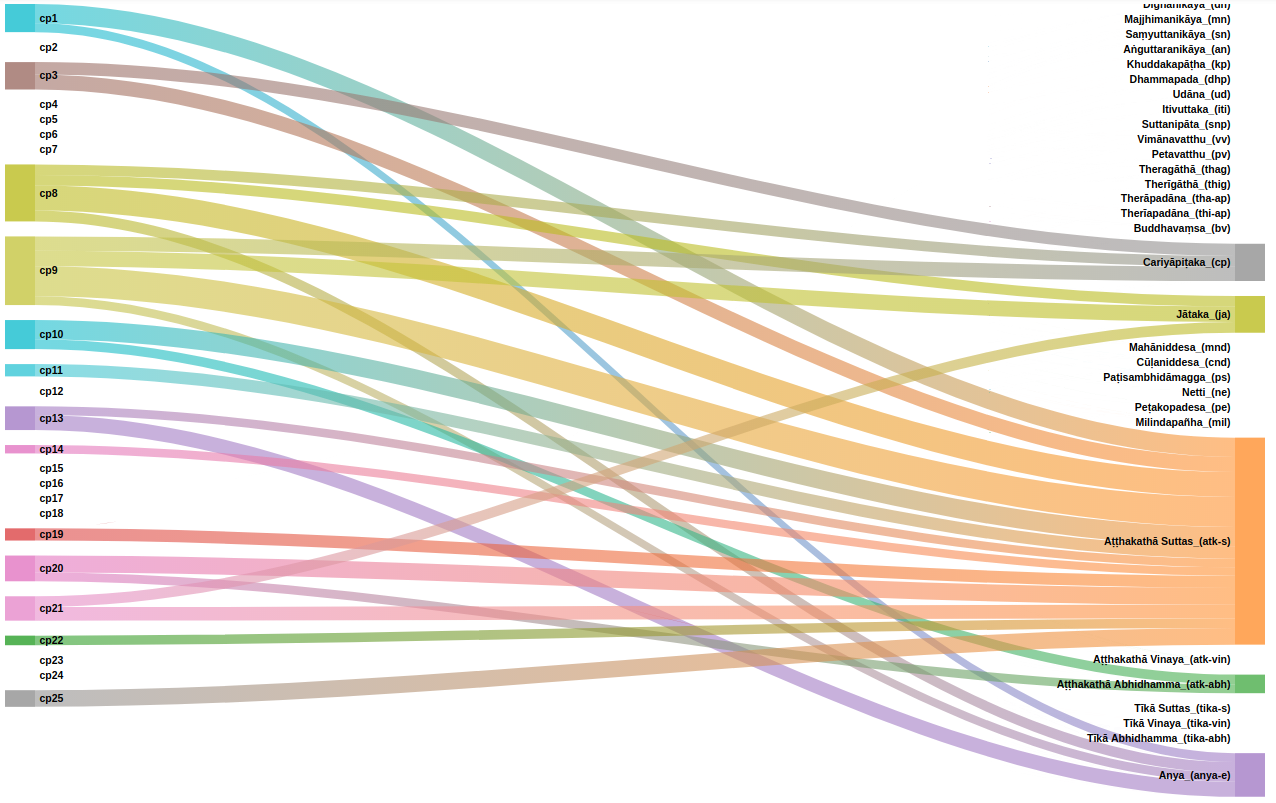
\includegraphics[width=\linewidth]{cp.png}
\captionof{figure}{Cariyāpiṭaka sankey chart showing connections with other collections}
\label{cp}

\medskip
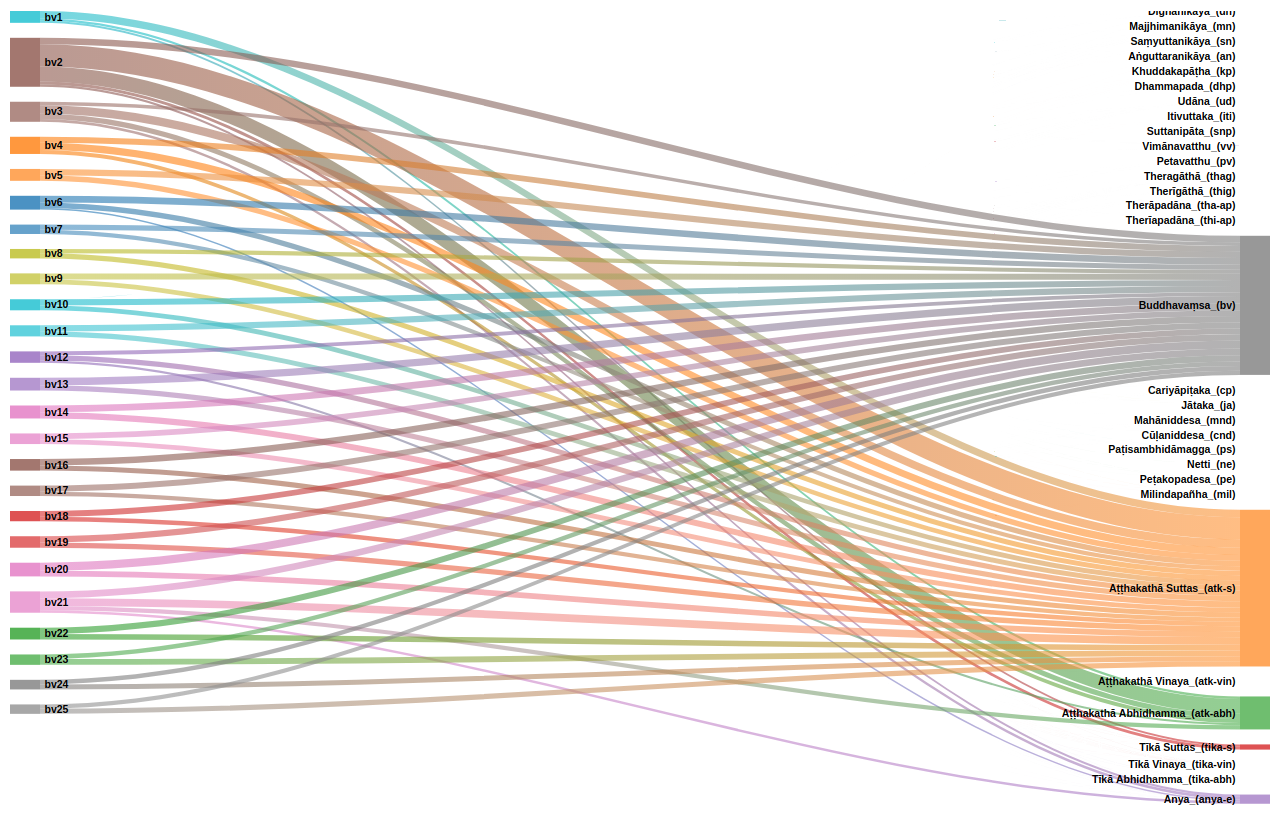
\includegraphics[width=\linewidth]{bv.png}
\captionof{figure}{Buddhavaṃsa sankey chart showing connections with other collections}
\label{bv}

\medskip
Note that the Buddhavaṃsa seems to be highly repetitive across the various texts in this collection.

The only matches found are with the commentaries and most notably with the Aṭṭhakathā Suttas. The major commentaries were based on earlier ones, now lost, in Prakrit and Sinhala, which were written down at the same time as the Canon, in the last century BCE. Would it be possible therefore that the Cariyāpiṭaka and Buddhavaṃsa were part of the lost early commentaries?

\subsubsection{Paṭisambhidāmagga (ps)}
The Paṭisambhidāmagga is an advanced critical treatise in thirty chapters on Buddhist practice. It is more reminiscent of the Abhidhamma and indeed this shows in it's very high AWL value. It does not have any counterparts in the northern canons.

The AWL value is however higher than most Abhidhamma collections so it might be possible that this text has developed in a very late stage.

\subsubsection{Peṭakopadesa (pe)}
The Peṭakopadesa is a systematic treatise intended to provide a guide for reading and interpreting the texts of the nikāyas. The Pali text of the Peṭakopadesa is quite corrupt, which is unusual in the Pali canon. It is a late text, lacking counterparts in the northern collections. It is not universally accepted as canonical; the Mahāsaṅgīti edition, which as a Burmese text, includes it.

As this text is not universally accepted as canonical, I will disregard the low value of the AWL as an anomaly.

\subsubsection{Bhikkhunī Pātimokkha (pli-tv-bi-pm)}
The AWL of the Bhikkhunī Pātimokkha seems very high in comparison to the other collections of the Vinaya. This is not surprising if we remember that the Bhikkhunī Pātimokkha had been lost and was actually reconstructed from a commentarial text. No doubt due to it's history, the text would also have acquired some of it's later use of the Pali language, most notably with concatted and therefore longer words. This does not say anything about the actual age of the original Bhikkhunī Pātimokkha, only of the current version we have.

\subsubsection{Parivāra (pli-tv-pvr)}
The Parivāra is a technical analysis of the content of the Suttavibhaṅga and the Khandhakas. The Parivāra is unique to the Theravada school and it is probable that it was compiled in the sectarian period. Its manner of analysis shares certain characteristics with the Abhidhamma.

The high value of the AWL is consistent with the idea that this is a later text. It is clearly compiles after the Suttavibhaṅga and the Khandhakas and has a higher AWL than both of these.

\subsubsection{Dhammasaṅgaṇī (ds)}
The Dhammasaṅgaṇī is the first book of the Abhidhamma and the low AWL value seems to have more to do with the structure of this book then it's age. The book is made up of mātikā, a lists of contents or matrix and is therefore a vastly different way of writing than verse or prose.

\subsubsection{Vibhaṅga (vb)}
The Vibhaṅga, unlike the Dhammasaṅgaṇī, seems to have a much greater AWL then most of the other Abhidhamma books. 

An overview of all the matches of this text with other texts reveals the connection with the suttas as well as other Abhidhamma texts, most notably the Dhammasaṅgaṇī. This does not explain the hight AWL other than that it is obviously later than the Dhammasaṅgaṇī itself.\\

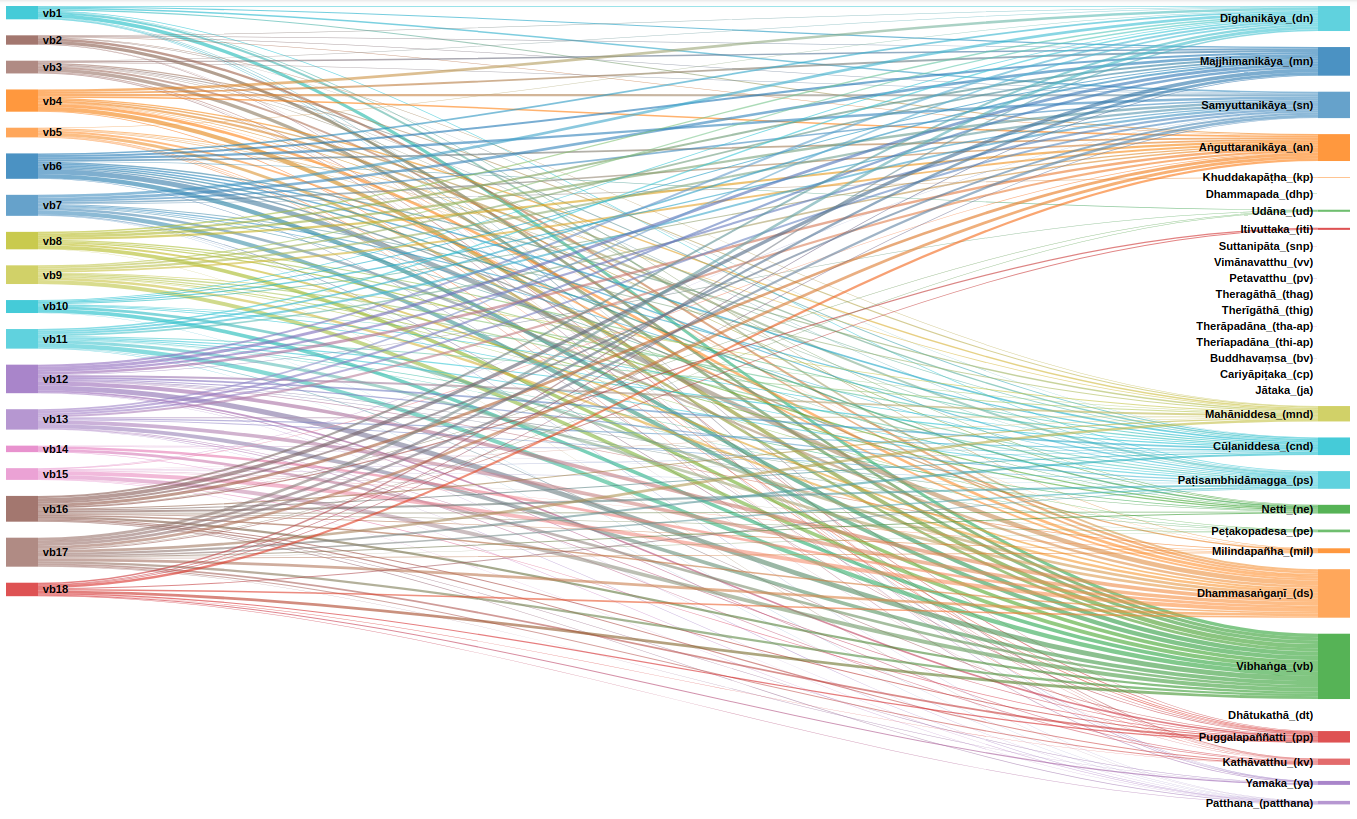
\includegraphics[width=\linewidth]{vbmatches.png}
\captionof{figure}{Sankey chart of all matches between the Vibhaṅga and other texts}
\label{vbmatches}

\subsubsection{Paṭṭhāna (patthana)}
The Paṭṭhāna has the largest AWL of all the Abhidhamma books. This book creates a huge complex structure of possible combinations based on the Dhammasaṅgaṇī and is heavily abbreviated. It is a work in itself and although it draws on the Dhammasaṅgaṇī, the main bulk of the text is unique in that it does not have many connections with other texts. Most notably, the text it has most matches with outside itself is the Parivāra.\\

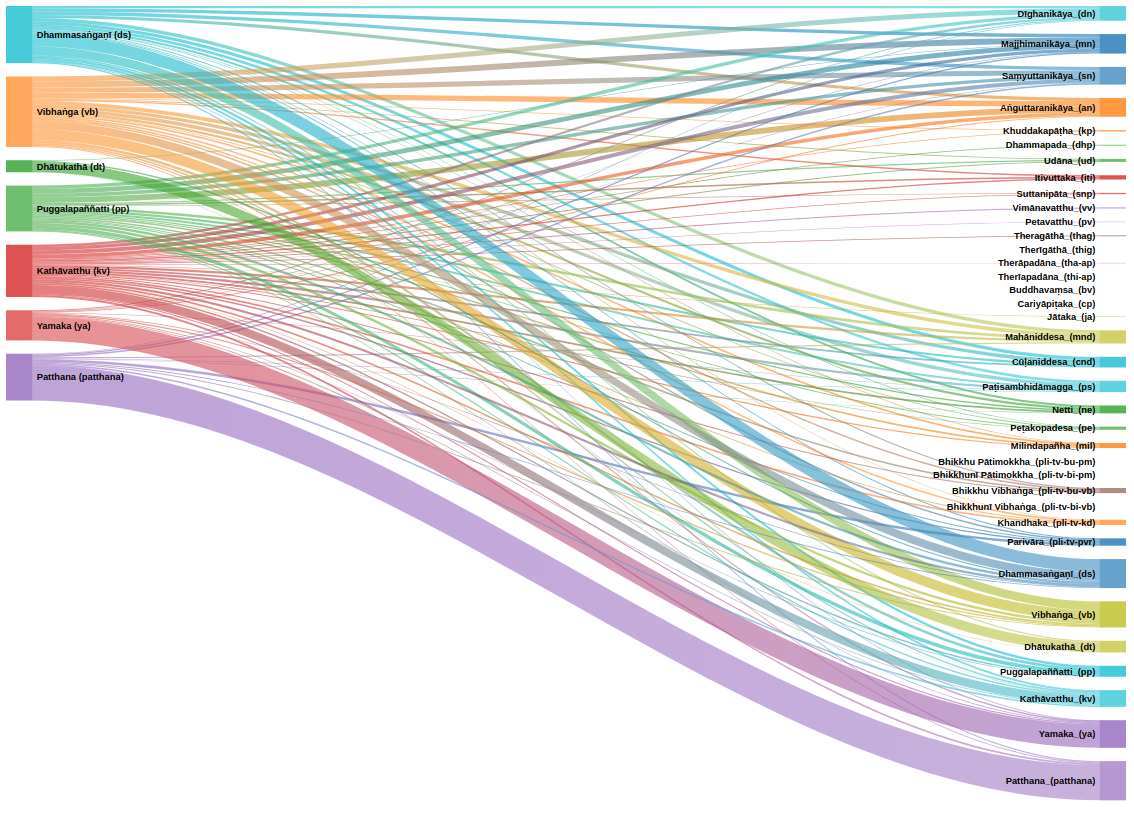
\includegraphics[width=\linewidth]{abhidhamma.png}
\captionof{figure}{Sankey chart of all matches between the Abhidhamma collections and other texts}
\label{abhidhamma}

\medskip
This figure also shows that all Abhidhamma collections are highly repetitive, given the high number of matches between the various chapters.

The Paṭṭhāna finds itself at the end of the Abhidhamma collection and with such a high AWL, I would consider it the latest book of the Abhidhamma, probably close to or overlapping with the development of the commentaries.

\subsubsection{Aṭṭhakathā (atk)}
The Aṭṭhakathā is a collection of Theravadin Buddhist commentaries to the canonical Theravadin Tipitaka. As noted before, the major commentaries were based on earlier ones, now lost, in Prakrit and Sinhala, which were written down at the same time as the Canon, in the last century BCE. Some material in the commentaries is found in canonical texts of other schools of Buddhism, suggesting an early common source. This can also explain why the AWL value of the Aṭṭhakathā on Suttas and Vinaya are relatively low and more in line with the other late texts like the Vinaya and Abhidhamma.

The contents of collected editions of the Theravadin commentaries, compiled from the fourth century CE onwards, varies between editions. 
\newpage
\bibliographystyle{plainnat}
\bibliography{bib}

% \setlength{\tabcolsep}{1.5em}
% % %\input{Chapters/glossar.tex}
% %  \printshorthands[title={Reference Literature}, keyword=sec, env=myshorthands_sec]
% %  \addcontentsline{toc}{section}{Reference Literature}

%  % additional material for the Appendix can go here.
%  % \newpage
%  % \section*{Appendix}
%  % \addcontentsline{toc}{section}{Appendix}


\end{document}

%%% Local Variables:
%%% mode: latex
%%% TeX-master: t
%%% End:
